% ============================================================
%  SCHOLA DOMESTICA — Magister Mathematica
%  Level 1 | Week 5 | Day 2
%  Topic: Comparing Numbers 0–10 with < > =
%  Enrichment: Roman Numerals VI–X (matching)
% ============================================================
\documentclass[12pt, letterpaper]{article}

\usepackage[top=1in, bottom=1in, left=1in, right=1in]{geometry}
\usepackage{fontenc}
\usepackage{inputenc}
\usepackage{lmodern}
\usepackage{microtype}
\usepackage{amsmath}
\usepackage{graphicx}
\usepackage{xcolor}
\usepackage{tikz}
\usepackage{array}
\usepackage{booktabs}
\usepackage{enumitem}
\usepackage{multicol}
\usepackage{mdframed}
\usepackage{fancyhdr}

\definecolor{scholared}{RGB}{160,30,30}
\definecolor{scholagold}{RGB}{180,140,40}
\definecolor{scholacream}{RGB}{253,248,235}
\definecolor{scholagreen}{RGB}{50,110,60}
\definecolor{scholablue}{RGB}{40,80,140}

\pagestyle{fancy}
\fancyhf{}
\renewcommand{\headrulewidth}{0.6pt}
\fancyhead[L]{\small\textcolor{scholared}{\textbf{Schola Domestica — Magister Mathematica}}}
\fancyhead[R]{\small\textcolor{scholared}{Level 1 · Week 5 · Day 2}}
\fancyfoot[C]{\small\textcolor{gray}{— \thepage\ —}}

\newcommand{\answerline}{\underline{\hspace{2.5cm}}}
\newcommand{\biganswerline}{\underline{\hspace{4cm}}}
\newcommand{\symbox}{\fbox{\hspace{0.7cm}}}  % box for < > =

\newmdenv[
  backgroundcolor=scholacream,
  linecolor=scholared,
  linewidth=1.5pt,
  roundcorner=6pt,
  innertopmargin=8pt,
  innerbottommargin=8pt,
  innerleftmargin=10pt,
  innerrightmargin=10pt
]{lessonbox}

\begin{document}

\begin{center}
  {\LARGE\textbf{\textcolor{scholared}{Comparing Numbers 0–10}}}\\[4pt]
  {\Large\textcolor{scholagold}{\textit{Using $<$, $>$, and $=$}}}\\[6pt]
  {\small Name: \biganswerline \hspace{1cm} Date: \answerline}
\end{center}

\vspace{4pt}
\noindent\textcolor{scholared}{\rule{\linewidth}{1pt}}
\vspace{4pt}

% ===== INSTRUCTION BOX =====
% IMAGE PROMPT (Beatrix Potter watercolour style):
% Two lily pads side by side on a still pond. On the left lily pad sit 9 small green frogs;
% on the right lily pad sit 6 frogs. Soft blue-green watercolour, morning light, white background.
% No text in the image.

\begin{lessonbox}
\textbf{The Alligator Rule:}\\[4pt]
The symbols $<$ and $>$ look like an alligator's open mouth.\\
The alligator \textbf{always eats the bigger number!}\\[6pt]
\begin{center}
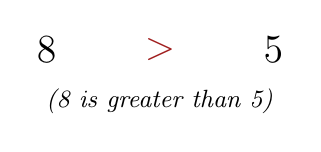
\begin{tikzpicture}[scale=1.2]
  \node at (0,0) {\Large $8$};
  \node at (1.2,0) {\Large\textcolor{scholared}{$>$}};
  \node at (2.4,0) {\Large $5$};
  \node at (1.2,-0.55) {\small\textit{(8 is greater than 5)}};
\end{tikzpicture}
\hspace{1.5cm}
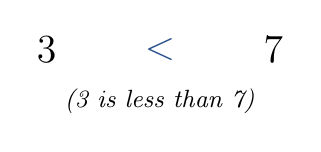
\begin{tikzpicture}[scale=1.2]
  \node at (0,0) {\Large $3$};
  \node at (1.2,0) {\Large\textcolor{scholablue}{$<$}};
  \node at (2.4,0) {\Large $7$};
  \node at (1.2,-0.55) {\small\textit{(3 is less than 7)}};
\end{tikzpicture}
\hspace{1.5cm}
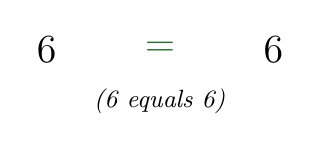
\begin{tikzpicture}[scale=1.2]
  \node at (0,0) {\Large $6$};
  \node at (1.2,0) {\Large\textcolor{scholagreen}{$=$}};
  \node at (2.4,0) {\Large $6$};
  \node at (1.2,-0.55) {\small\textit{(6 equals 6)}};
\end{tikzpicture}
\end{center}
\end{lessonbox}

\bigskip

% ===== PART I: WRITE < > = =====
\noindent\textcolor{scholared}{\large\textbf{Part I — Write $<$, $>$, or $=$}} \hfill \textit{(Problems 1–8)}

\medskip
\noindent\textit{Write the correct symbol in each box.}

\bigskip

\begin{multicols}{2}
\noindent\textbf{1.} \quad $6$ \quad \symbox \quad $9$ \\[18pt]
\noindent\textbf{2.} \quad $10$ \quad \symbox \quad $7$ \\[18pt]
\noindent\textbf{3.} \quad $8$ \quad \symbox \quad $8$ \\[18pt]
\noindent\textbf{4.} \quad $0$ \quad \symbox \quad $6$

\columnbreak

\noindent\textbf{5.} \quad $7$ \quad \symbox \quad $9$ \\[18pt]
\noindent\textbf{6.} \quad $10$ \quad \symbox \quad $10$ \\[18pt]
\noindent\textbf{7.} \quad $6$ \quad \symbox \quad $7$ \\[18pt]
\noindent\textbf{8.} \quad $9$ \quad \symbox \quad $6$
\end{multicols}

\bigskip
\noindent\textcolor{scholared}{\rule{\linewidth}{0.4pt}}

% ===== PART II: CIRCLE THE BIGGER NUMBER =====
\noindent\textcolor{scholared}{\large\textbf{Part II — Circle the Greater Number}} \hfill \textit{(Problems 9–12)}

\bigskip
\begin{multicols}{2}
\noindent\textbf{9.} \quad

\begin{tikzpicture}[baseline=-0.5ex]
  \draw[thick] (0,0) circle (0.4cm); \node at (0,0) {\Large 6};
\end{tikzpicture}
\quad or \quad

\begin{tikzpicture}[baseline=-0.5ex]
  \draw[thick] (0,0) circle (0.4cm); \node at (0,0) {\Large 8};
\end{tikzpicture}\\[18pt]

\noindent\textbf{10.} \quad

\begin{tikzpicture}[baseline=-0.5ex]
  \draw[thick] (0,0) circle (0.4cm); \node at (0,0) {\Large 9};
\end{tikzpicture}
\quad or \quad

\begin{tikzpicture}[baseline=-0.5ex]
  \draw[thick] (0,0) circle (0.4cm); \node at (0,0) {\Large 7};
\end{tikzpicture}

\columnbreak

\noindent\textbf{11.} \quad

\begin{tikzpicture}[baseline=-0.5ex]
  \draw[thick] (0,0) circle (0.4cm); \node at (0,0) {\Large 10};
\end{tikzpicture}
\quad or \quad

\begin{tikzpicture}[baseline=-0.5ex]
  \draw[thick] (0,0) circle (0.4cm); \node at (0,0) {\Large 9};
\end{tikzpicture}\\[18pt]

\noindent\textbf{12.} \quad

\begin{tikzpicture}[baseline=-0.5ex]
  \draw[thick] (0,0) circle (0.4cm); \node at (0,0) {\Large 0};
\end{tikzpicture}
\quad or \quad

\begin{tikzpicture}[baseline=-0.5ex]
  \draw[thick] (0,0) circle (0.4cm); \node at (0,0) {\Large 7};
\end{tikzpicture}
\end{multicols}

\bigskip
\noindent\textcolor{scholared}{\rule{\linewidth}{0.4pt}}

% ===== PART III: WORD PROBLEMS =====
\noindent\textcolor{scholared}{\large\textbf{Part III — Think About It}} \hfill \textit{(Problems 13–14)}

\bigskip
\noindent\textbf{13.} Anna has 8 cherries. Boris has 6 cherries. Who has \textbf{more}? \hfill \answerline

\bigskip
\noindent How many \textbf{fewer} does Boris have? \hfill \answerline

\bigskip\bigskip
\noindent\textbf{14.} A cat catches 9 mice on Monday and 9 mice on Tuesday.\\[4pt]
Are the two days the \textbf{same}, or is one day \textbf{more}? \hfill \answerline

\bigskip
\noindent Write a comparison: \quad $9$ \quad \symbox \quad $9$

\bigskip
\noindent\textcolor{scholared}{\rule{\linewidth}{0.4pt}}

% ===== ENRICHMENT =====
\begin{lessonbox}
\textcolor{scholared}{\textbf{Enrichment — Roman Numerals: Match the Symbols}}\\[6pt]
\noindent Draw a line to match each Roman numeral to its number.\\[8pt]
\begin{center}
\begin{tabular}{p{2cm} p{3cm} p{2cm}}
  \textbf{VI}   & \hspace{1cm} & 10 \\[6pt]
  \textbf{VII}  & \hspace{1cm} & 7  \\[6pt]
  \textbf{VIII} & \hspace{1cm} & 9  \\[6pt]
  \textbf{IX}   & \hspace{1cm} & 6  \\[6pt]
  \textbf{X}    & \hspace{1cm} & 8  \\
\end{tabular}
\end{center}
\medskip
\noindent\textit{Bonus:} Write I through X in Roman numerals: \quad \answerline
\end{lessonbox}

\end{document}
